\documentclass{article}
\usepackage{graphicx}
\usepackage{float}
\title{Labwork 2: Linear Regression}
\author{Tran The Trung}
\begin{document}
\maketitle

\section{Implementation}
The full implementation of the code could be seen in figure \ref{fig:code}. Here we make the same implementation as the Gradient Descent but extend it to two derivative functions, one for $w0$, one for $w1$. For each loop, we need to calculate the gradient for $w0$ and $w1$ which is the averaged gradient for each data samples. Afterwards we can update the weights based on these new gradients and calculate a new loss value.

\begin{figure}[H]
    \centering
    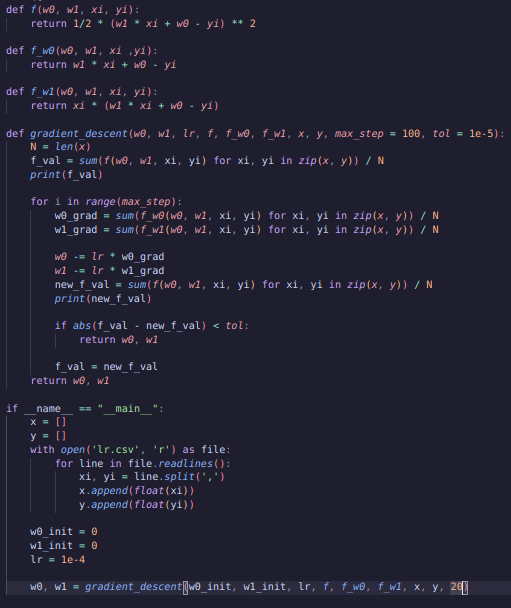
\includegraphics[width=0.68\linewidth]{image/code.png}
    \caption{Linear Regression Implementation}
    \label{fig:code}
\end{figure}

For this problem, we use simple data for house price prediction problem. The data consists of only one feature which is the area and only 5 samples. Using the above implementation, the final result for this linear regression could be seen in figure \ref{fig:vis} where we can see the final prediction line is fitting quite well with all the data points.

\begin{figure}[H]
    \centering
    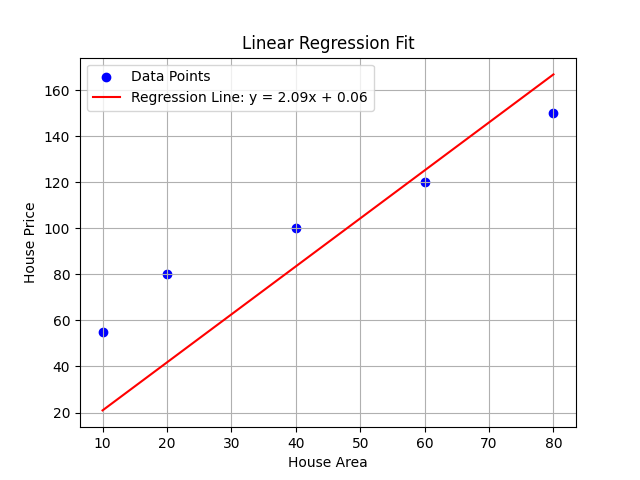
\includegraphics[width=0.8\linewidth]{image/regression.png}
    \caption{Result Visualization}
    \label{fig:vis}
\end{figure}

\section{Analysis of learning rate effect}
Here in this section, we could make some small tests on the effect of different learning rate to the final result. 

\begin{figure}[H]
    \centering
    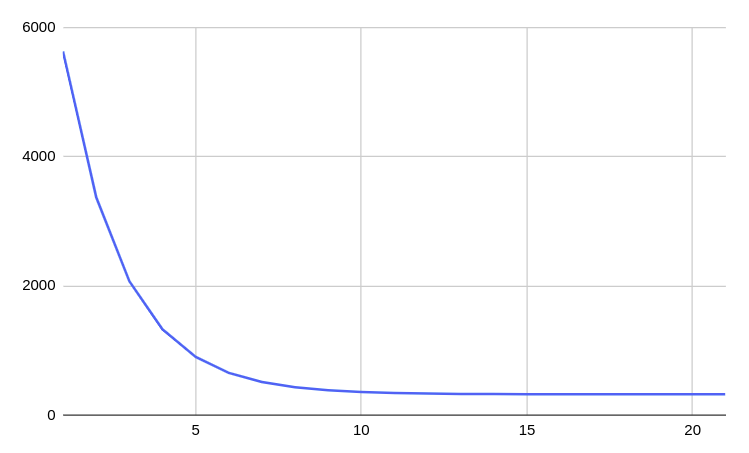
\includegraphics[width=0.75\linewidth]{image/lr01.png}
    \caption{Learning rate = $10^-4$}
    \label{fig:lr01}
\end{figure}


\begin{figure}[H]
    \centering
    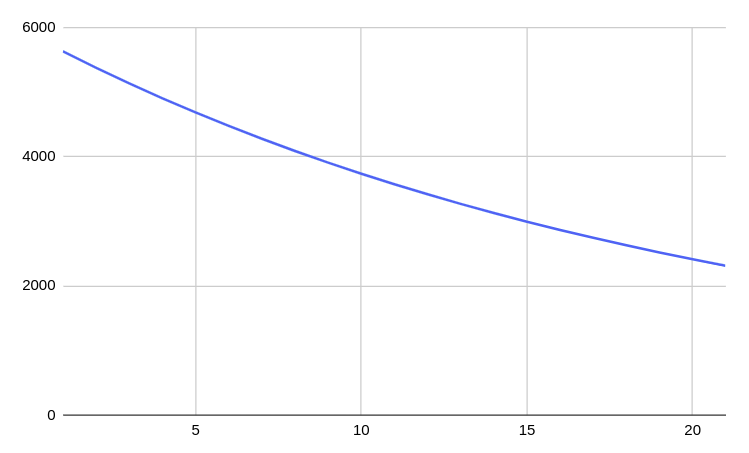
\includegraphics[width=0.75\linewidth]{image/lr11.png}
    \caption{Learning rate = $10^-5$}
    \label{fig:lr001}
\end{figure}

\begin{figure}[H]
    \centering
    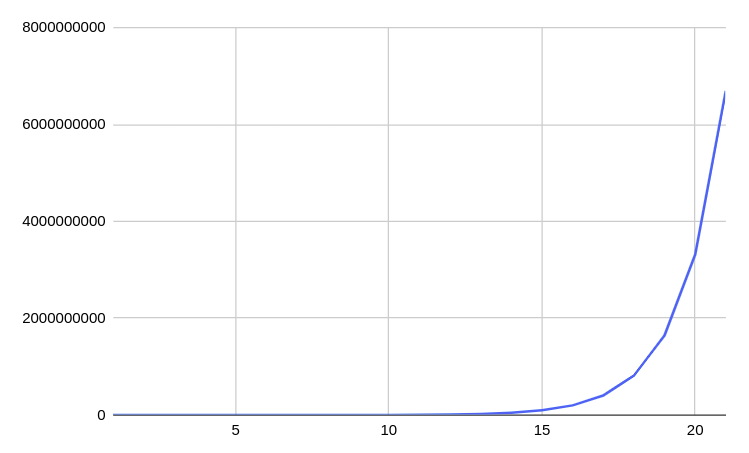
\includegraphics[width=0.75\linewidth]{image/lr001.png}
    \caption{Learning rate = $10^-3$}
    \label{fig:lr11}
\end{figure}


We make three scenarios according to three different values of learning rate: $10^-3$, $10^-4$ and $10^-5$. As discussed in the previous labwork, the choice of learning rate is critical in training deep learning models. A learning rate that is too high (as shown in Figure \ref{fig:lr11}) can cause the model to diverge, while a learning rate that is too low (as shown in figure \ref{fig:lr001} may result in extremely slow convergence or even cause the model to get stuck at saddle points. This experiment further highlights that the optimal learning rate can vary significantly depending on the specific problem, and therefore, making experimentation is often necessary to determine the most suitable value.

\end{document}